\documentclass[]{article}
\usepackage{mathtools}
\usepackage{amsmath}
\usepackage{graphicx}
\usepackage{xspace}
\usepackage{float}
\usepackage{tikz}
\graphicspath{ {Afbeeldingen/} }

%opening
\title{
Laboverslag Signaalverwerking \\ 
\begin{large} 
Opgave1: Analyse van een actieve filtertrap
\end{large} }
\author{Van Dessel Stijn}

\begin{document}

\maketitle

\section{Specificaties}

\begin{tabular}{ l l }
Type filter 			&  Band Pass (Akerberg-Mossberg)-inverting (Schema 21)\\
Amplituderesponsie 		&  $|H|_{max}$ = 6dB  \\
						&  $|H(10 KHz)|$ = -26dB  \\
Kwaliteitsfactor polen 	&  $Q_p$ = 4  \\
\end{tabular}


\begin{figure}[h]
\centering
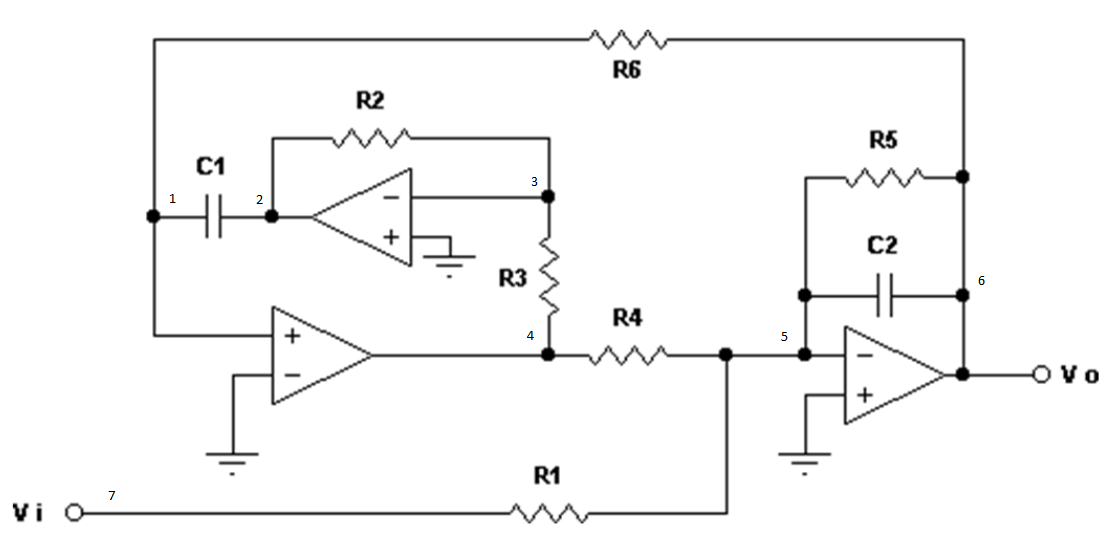
\includegraphics[scale=0.4]{schema}
\caption{Band Pass (Akerberg-Mossberg)-inverting}
\label{fig:schema}
\end{figure}


\section{Analyse}

\subsection*{Bepalen HF en DC weergave}

\subsubsection*{DC}

Bij DC vormen de condensatoren een open verbinding. Dit resulteert in volgend
principeschema. Doordat C1 voor een open verbinding zorgt, zal deze feedback
loop wegvallen en zal er uiteindelijk een verzwakking optreden.

\begin{equation*}
\boxed{|H|_{DC} = -\infty dB}
\end{equation*}

\begin{figure}[H]
	\centering
	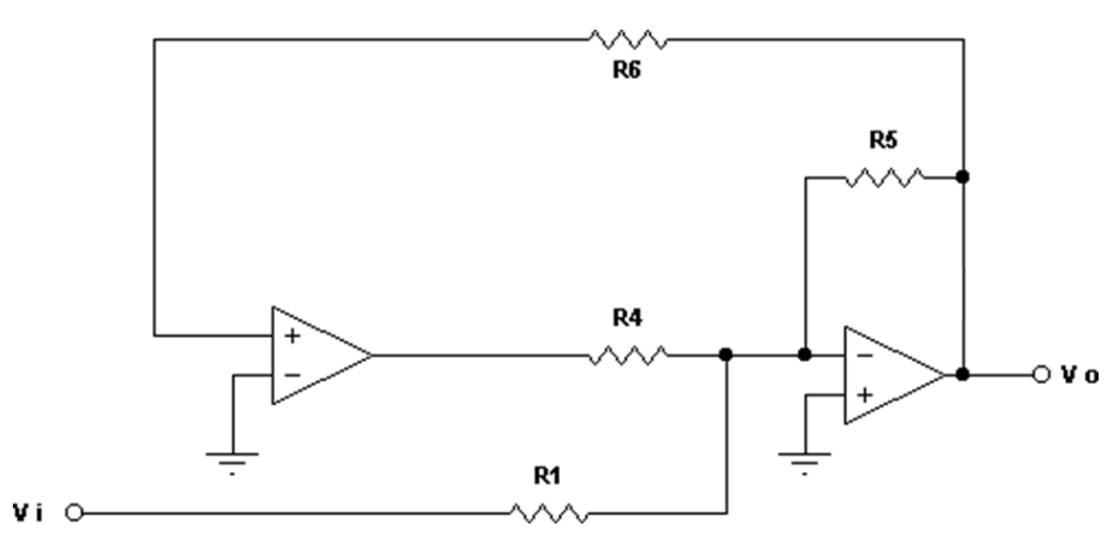
\includegraphics[scale=0.35]{schema_DC}
	\caption{Principeschema DC-weergave H(0)}
	\label{fig:schema_DC}
\end{figure}

\subsubsection*{HF}

Bij HF zullen de condensatoren een doorverbinding of kortsluiting vormen. Dit
resulteert in onderstaand principeschema. De condensator C2 zorgt hier bij de
terugkoppeling voor een zeer kleine weerstand. Hierdoor kunnen we stellen dat
de uiteindelijke versterking bij HF kleiner dan 1 zal zijn. Hierdoor zal er dan
ook een grote verzwakking optreden bij HF.

\begin{equation*}
	\boxed{|H|_{HF} = -\infty dB}
\end{equation*}


\begin{figure}[H]
	\centering
	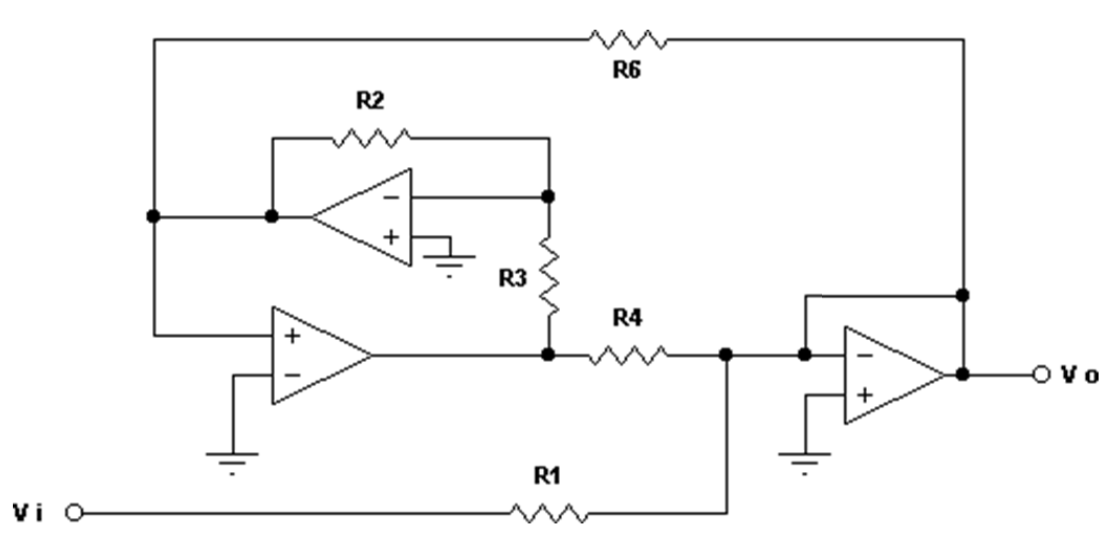
\includegraphics[scale=0.35]{schema_hf}
	\caption{Principeschema DC-weergave H(0)}
	\label{fig:schema_HF}
\end{figure}

\subsection*{Berekenen transferfunctie}

De correcte transferfunctie werdt niet bekomen.

\begin{equation*}
H(s) = \cfrac{V_{o}}{V_{i}}
\end{equation*}

Stroom door $ C_{1} = R_{6} $
en stroom door $ R_{3} = R_{2} $

\subsubsection*{Stroom knooppunt 1}

\begin{equation*}
0 = \cfrac{V_{2}-0}{R_{3}} + \cfrac{V_{3}-0}{R_{2}} = \cfrac{V_{2}}{R_{3}} + \cfrac{V_{3}}{R_{2}}
\end{equation*}

\subsubsection*{Stroom knooppunt 2}

\begin{equation*}
0 = \cfrac{V_{3}-0}{\cfrac{1}{sC_{1}}} + \cfrac{V_{1}-0}{R_{6}} = sC_{1}V_{3} + \cfrac{V_{1}}{R_{6}}
\end{equation*}

\subsubsection*{Stroom knooppunt 3}

\begin{equation*}
0 = \cfrac{V_{1}}{R_{5}}+\cfrac{V_{1}}{\cfrac{1}{sC_{2}}}+\cfrac{V_{2}}{R_{4}}+\cfrac{V_{i}}{R_{1}} = \cfrac{V_{1}}{R_{5}}+sC_{2}V_{1}+\cfrac{V_{2}}{R_{4}}+\cfrac{V_{i}}{R_{1}} 
\end{equation*}


\subsection*{Vergelijken transfer functie met de algemene transferfunctie}

\subsubsection*{Algemene transferfunctie}
\begin{equation*}
H(\omega) = K 
\cfrac
{(\cfrac{s}{\omega_{nz}})^{2}+\cfrac{1}{Q_{z}}(\cfrac{s}{\omega_{nz}})+1}
{(\cfrac{s}{\omega_{np}})^{2}+\cfrac{1}{Q_{p}}(\cfrac{s}{\omega_{np}})+1}
\end{equation*}

\subsubsection*{Transferfunctie}
\begin{equation*}
H(\omega) = -	\cfrac{R_{5}}{R_{1}} 
\cfrac{sC_{1}R_{2}R_{4}R_{6}/R_{3}R_{5}}
{s^{2}C_{1}C_{2}R_{2}R_{4}R_{6}/R_{3}+sC_{1}R_{2}R_{4}R_{6}/R_{3}R_{5}+1}
\end{equation*}

\subsubsection*{Karakteriseren}
\begin{equation*}
K = -	\cfrac{R_{5}}{R_{1}} 
\end{equation*}

\begin{equation*}
(\cfrac{1}{\omega_{np}})^{2} = (\cfrac{1}{\omega_{nz}})^{2} = \cfrac{C_{1}C_{2}R_{2}R_{4}R_{6}}{R_{3}}
\end{equation*}

\begin{equation*}
\cfrac{1}{\omega_{np}Q_{p}} = \cfrac{1}{\omega_{nz}Q_{z}} = \cfrac{C_{1}R_{2}R_{4}R_{6}}{R_{3}R_{5}} 
\end{equation*}


\subsection*{Pole-zero plot}

Na analyse van de transfer functie kunnen we besluiten dat de filter beschikt over:

\begin{itemize}
	\item 1 Zero
	\item 2 Polen
\end{itemize}

\subsubsection*{Ligging zero's bepalen}

\begin{equation*}
\cfrac{s}{\omega_{nz}Q_{z}} = \cfrac{s}{4\times2\pi\times1000} = \cfrac{s}{4000\pi} = 0
\end{equation*}


\begin{equation*}
\boxed{s = 0 = transmissienulpunt(oorsprong)}
\end{equation*}

\subsubsection*{Ligging polen bepalen}

\begin{equation*}
(\cfrac{s}{\omega_{np}})^{2}+(\cfrac{s}{Q_{p}\omega_{np}})+1 = 0
\end{equation*}

\begin{equation*}
\cfrac{s^{2}}{(1000\times2\pi)^{2}} + \cfrac{s}{4\times1000\times2\pi} + 1 = 0
\end{equation*}

\begin{equation*}
\cfrac{s^{2}}{(2000\pi)^{2}} + \cfrac{s}{8000\pi} + 1 = 0
\end{equation*}

\begin{equation*}
\boxed{ s = 250(-1 \pm 3i\sqrt{7})\pi = $ 2 Complexe polen$}
\end{equation*}

\begin{equation*}
\boxed{ s = −785 \pm 6234i}
\end{equation*}

\begin{equation*}
\boxed{ s =  6283\angle\pm97^\circ}
\end{equation*}




\begin{figure}[H]
	\centering
	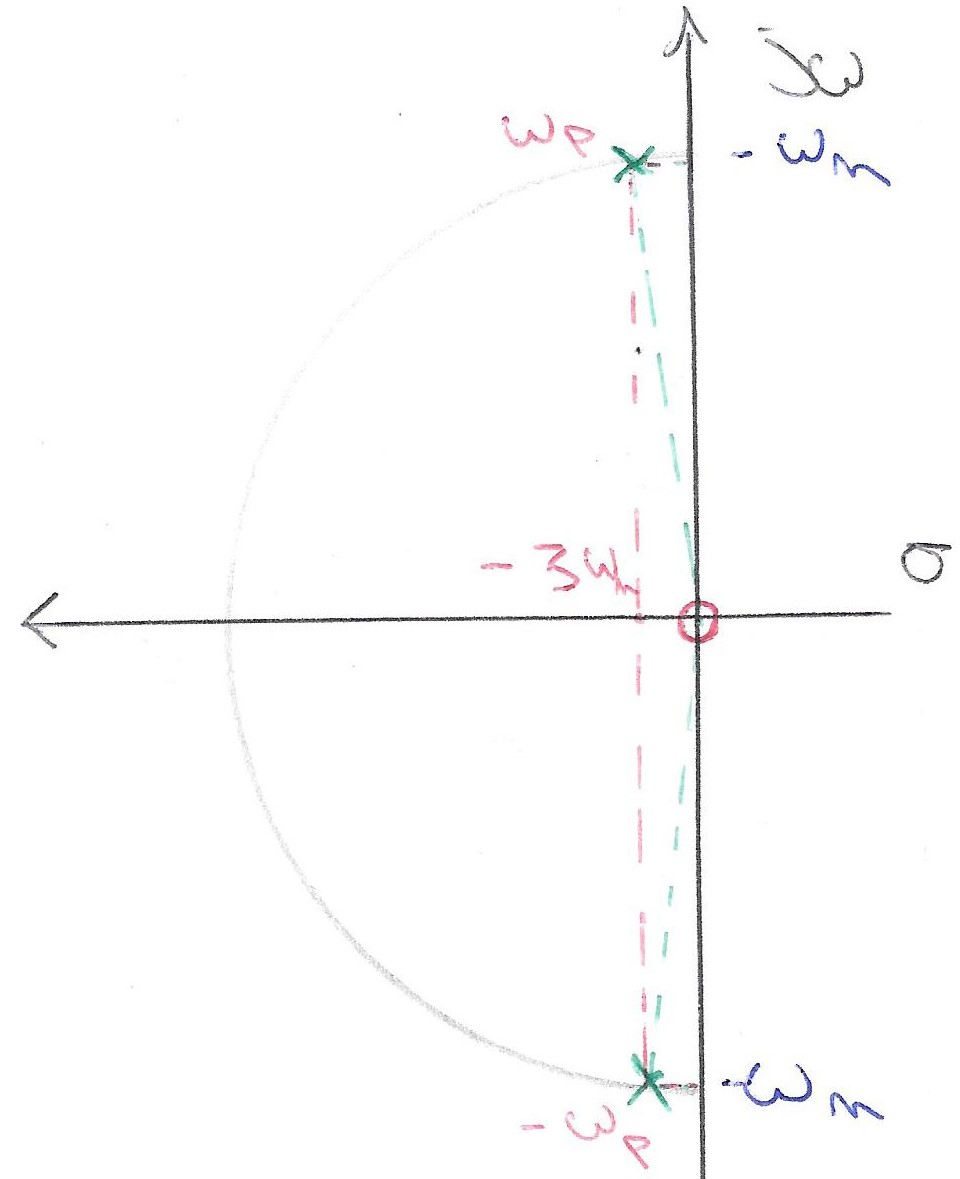
\includegraphics[scale=1.2]{schets_pz}
	\caption{Schets pole-zero map}
\end{figure}

\newpage

\subsection*{Bodediagram}

Als we het verband tussen het bodediagram en de pole-zero bekijken zien we de eigenschappen terug keren. Zo zien we dat de pole-zero map een 1 transmissie nulpunt heeft. Dit zal her voor zorgen da het bode diagram begint te stijgen vanaf DC met een helling van "+1". Als we hoger in frequentie kijken zien we 2 polen. Deze 2 samen zullen zorgen voor een helling van "-2", wat resulteert in een helling vanaf dit punt van "-1" of -20dB/dec.

\begin{figure}[H]
	\centering
	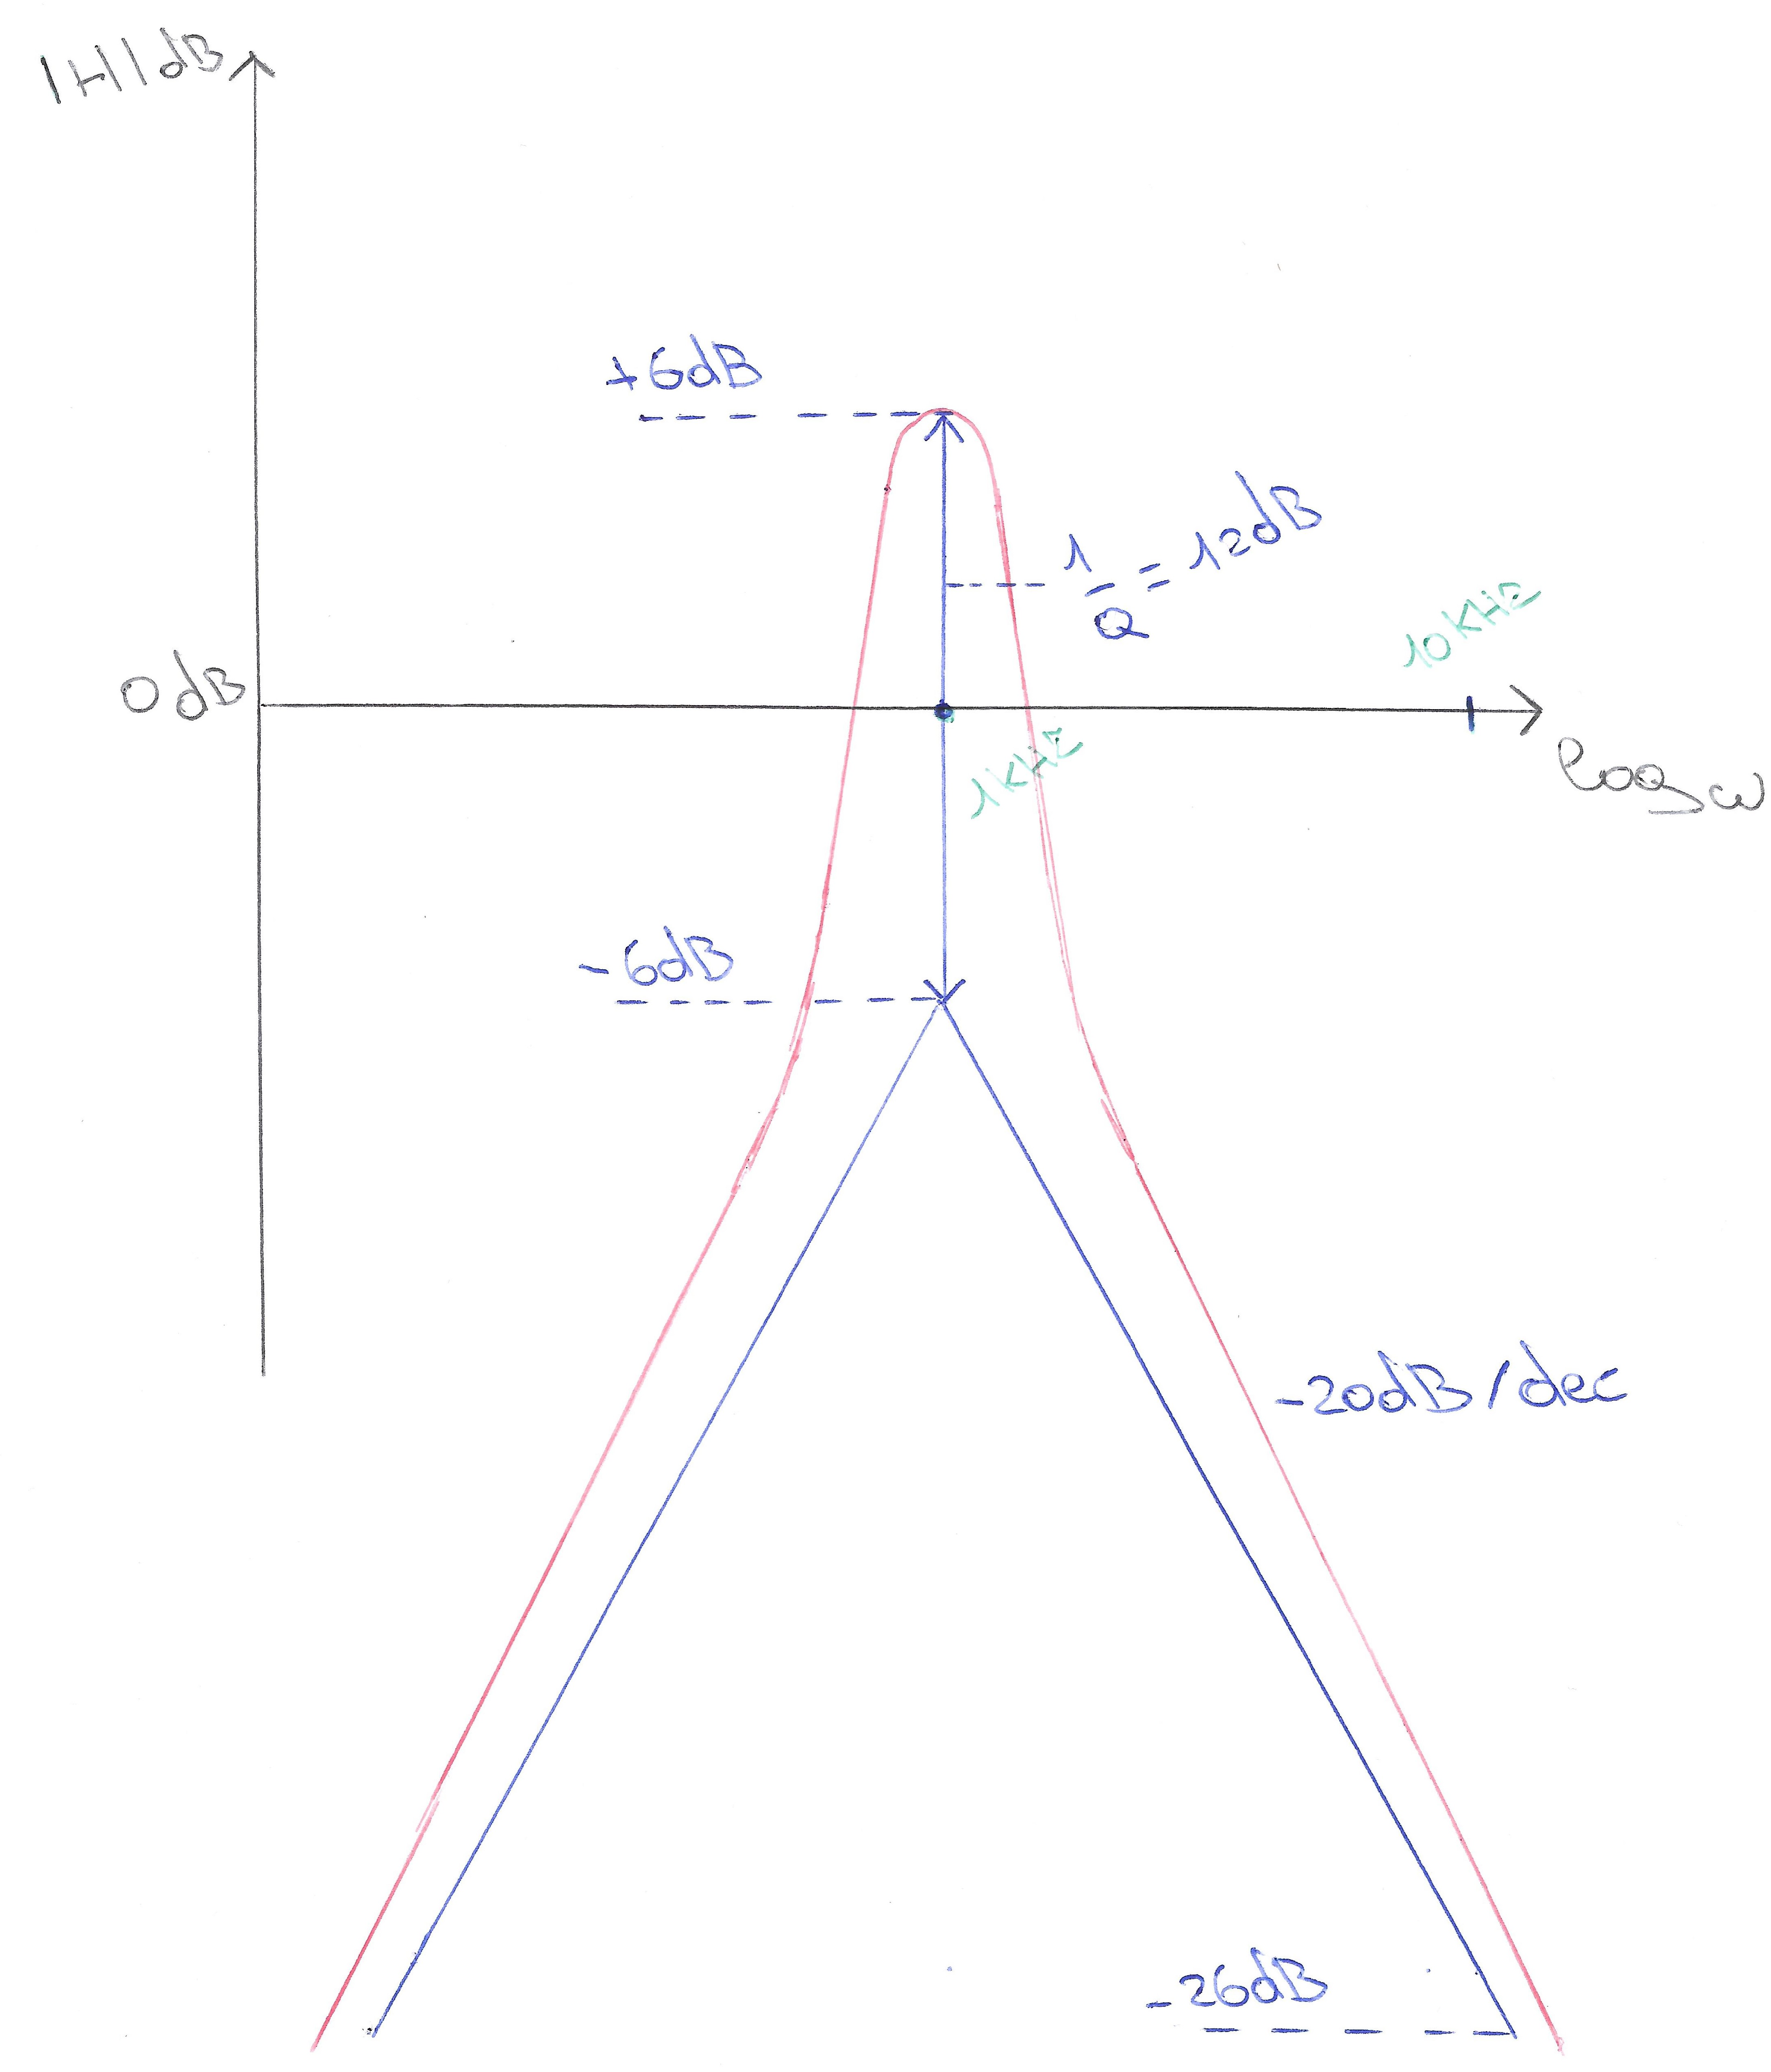
\includegraphics[width=12cm]{schets_bode}
	\caption{Schets bode diagram}
\end{figure}

\subsection*{Stapresponsie}

Als we de stapresponsie analyseren zien we dat deze zal starten op 0V. Dit doordat $|H|_{HF} = -\infty$ dB. Ook zal de stap uittrillen op 0V doordat $|H|_{DC} = -\infty$ dB. De gedempte sinus start naar beneden door het minteken voor de transferfunctie. De frequentie van het uittrillen zal gelijk zijn aan: 

\begin{equation*}
\boxed{ f_{p} =  \frac{\omega_{p}}{2\pi}}
\end{equation*}

Des te dichter dat een nulpunt tegen de $j\omega$ as liggen des de groter de demping van het systeem zal zijn. $\omega_{p}$ bepaald dan weer de frequentie van de uitslingering. De nulpunten in deze filter liggen dicht tegen de $j\omega$ as en zullen dus een grote demping hebben.


\begin{figure}[H]
	\centering
	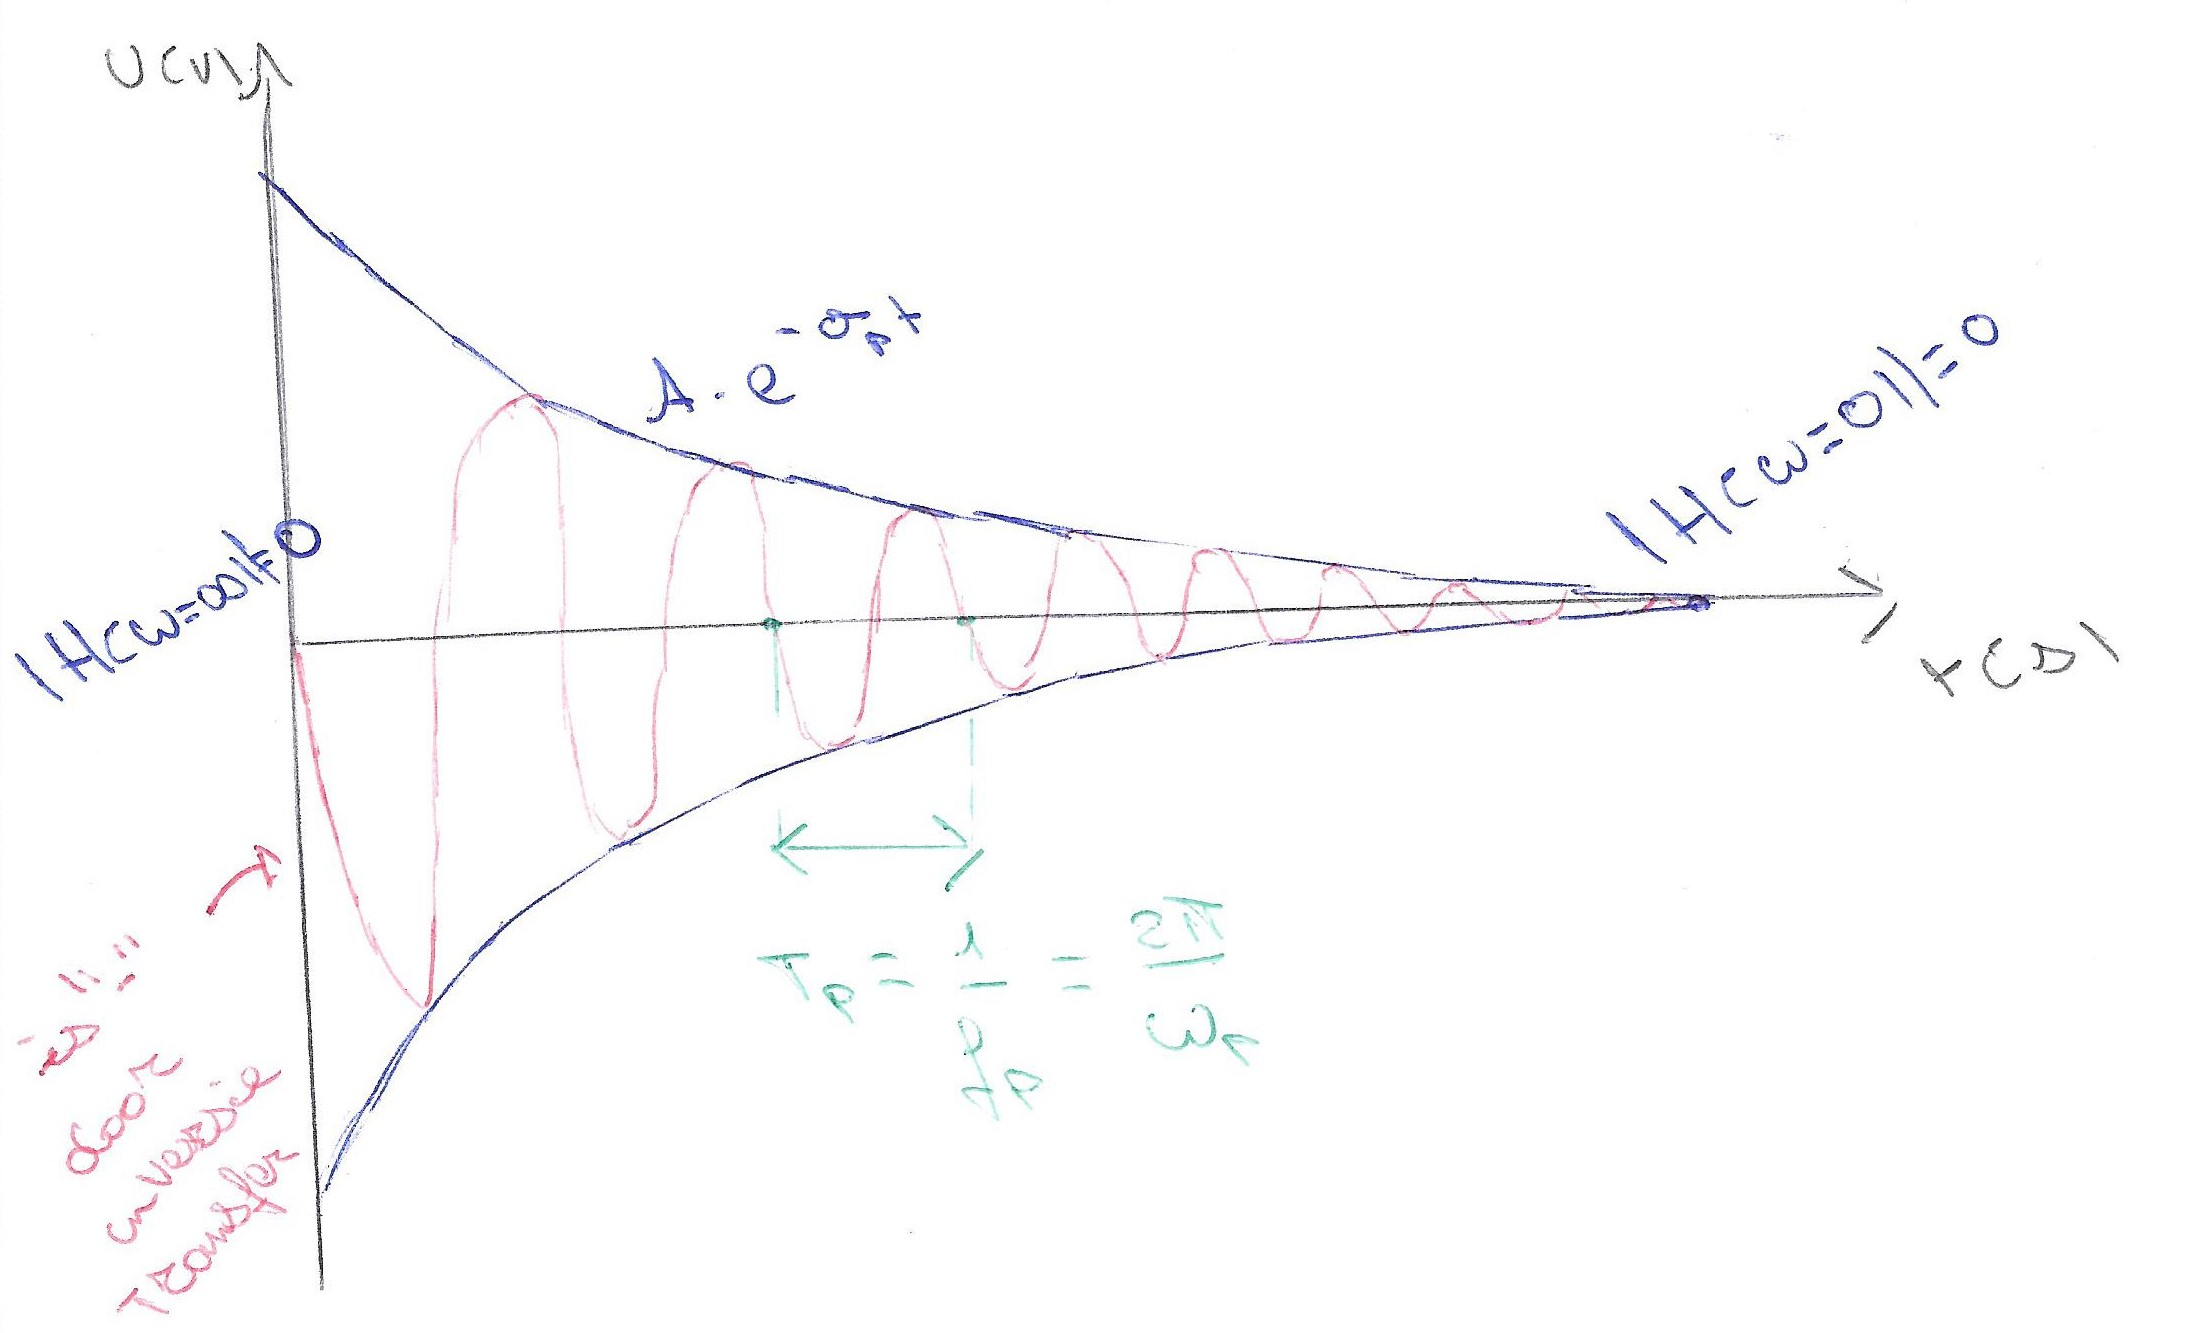
\includegraphics[width=13cm]{schets_step}
	\caption{Schets stapresponsie}
\end{figure}

\newpage

\section{Synthese}

\subsection*{Opstellen Ontwerpvergelijkingen}

Bij het opstellen van de ontwerpvergelijkingen worden enkel componentwaarden aan elkaar gelijk gesteld om zo het aantal vrijheidsgraden te beperken. Volgende veronderstellingen worden genomen:

\begin{equation*}
C_{1} = 1
\end{equation*}

\begin{equation*}
R_{1} = R_{2} = R_{3} = R_{4} = R_{6} = R
\end{equation*}

\begin{equation*}
R_{5} = ?
\end{equation*}

\begin{equation*}
C_{2} = ?
\end{equation*}



\subsubsection*{Algemene transferfunctie}
\begin{equation*}
H(\omega) = K 
\cfrac
{(\cfrac{s}{\omega_{nz}})^{2}+\cfrac{1}{Q_{z}}(\cfrac{s}{\omega_{nz}})+1}
{(\cfrac{s}{\omega_{np}})^{2}+\cfrac{1}{Q_{p}}(\cfrac{s}{\omega_{np}})+1}
\end{equation*}

\subsubsection*{Transferfunctie}
\begin{equation*}
H(\omega) = -	\cfrac{R_{5}}{R_{1}} 
				\cfrac{sC_{1}R_{2}R_{4}R_{6}/R_{3}R_{5}}
				{s^{2}C_{1}C_{2}R_{2}R_{4}R_{6}/R_{3}+sC_{1}R_{2}R_{4}R_{6}/R_{3}R_{5}+1}
\end{equation*}

\subsubsection*{1ste Ontwerpvergelijking}
\begin{equation*}
(\cfrac{1}{\omega_{np}})^{2} = \cfrac{C_{1}C_{2}R_{2}R_{4}R_{6}}{R_{3}} 
\end{equation*}

\begin{equation*}
(\cfrac{1}{\omega_{np}})^{2} = \cfrac{C_{1}C_{2}R_{2}R_{4}R_{6}}{R_{3}} 
\end{equation*}

\begin{equation*}
(\cfrac{1}{\omega_{np}})^{2} = \cfrac{C_{2}R^{3}}{R} 
\end{equation*}

\begin{equation*}
(\cfrac{1}{\omega_{np}})^{2} = {C_{2}R^{2}} 
\end{equation*}

\begin{equation} \label{eq:omega}
\boxed{\omega_{np} = \sqrt{\cfrac{1}{C_{2}R^{2}}}}
\end{equation}

\begin{equation} \label{eq:r}
\boxed{R = \sqrt{\cfrac{1}{\omega_{np}^{2}C_{2}}}}
\end{equation}

\begin{equation} \label{eq:c2}
\boxed{C_{2} = \cfrac{1}{\omega_{np}^{2}R^{2}}}
\end{equation}

\subsubsection*{2de Ontwerpvergelijking}
\begin{equation*}
\cfrac{1}{\omega_{np}Q_{p}} = \cfrac{C_{1}R_{2}R_{4}R_{6}}{R_{3}R_{5}} 
\end{equation*}

\begin{equation*}
\cfrac{1}{\omega_{np}Q_{p}} = \cfrac{R^{3}}{R_{5}R} 
\end{equation*}

\begin{equation*}
\cfrac{1}{\omega_{np}Q_{p}} = \cfrac{R^{2}}{R_{5}} 
\end{equation*}

\begin{equation} \label{eq:qp}
\boxed{Q_{p} = \cfrac{R_{5}}{R^{2}\omega_{np}}}
\end{equation}

\subsubsection*{3de Ontwerpvergelijking}

\begin{equation*}
K = \cfrac{R_{5}}{R} 
\end{equation*}

\begin{equation} \label{eq:r5}
\boxed{R_{5} = KR}
\end{equation}

\subsubsection*{4de Ontwerpvergelijking (\ref{eq:r5} in \ref{eq:qp})}

\begin{equation*}
Q_{p} = \cfrac{R_{5}}{\omega_{np}R^{2}}
\end{equation*}

\begin{equation*}
R^{2} = \cfrac{R_{5}}{\omega_{np}Q_{p}}
\end{equation*}

\begin{equation*}
R^{2} = \cfrac{KR}{\omega_{np}Q_{p}}
\end{equation*}

\begin{equation} \label{eq:R}
\boxed{R = \cfrac{K}{\omega_{np}Q_{p}}}
\end{equation}

\subsubsection*{5de Ontwerpvergelijking (\ref{eq:R} in \ref{eq:c2})}

\begin{equation*}
C_{2} = \cfrac{1}{\omega_{np}^{2}R^{2}}
\end{equation*}

\begin{equation*}
C_{2} = \cfrac{1}{\omega_{np}^{2}(\cfrac{K}{\omega_{np}Q_{p}})^{2}}
\end{equation*}

\begin{equation*}
C_{2} = \cfrac{1}{\omega_{np}^{2}\cfrac{K^{2}}{\omega_{np}^{2}Q_{p}^{2}}}
\end{equation*}

\begin{equation*}
C_{2} = \cfrac{1}{\cfrac{K^{2}}{Q_{p}^{2}}}
\end{equation*}

\begin{equation*}
C_{2} = \cfrac{Q_{p}^{2}}{K^{2}}
\end{equation*}

\begin{equation}
\boxed{C_{2} = (\cfrac{Q_{p}}{K})^{2}}
\end{equation}

\newpage

\subsection*{Berekenen componentwaarden}

Met de bekomen ontwerpvergelijkingen uit vorige paragraaf kunnen nu de componentwaarden berekend worden. De berekende waarden zijn theoretische waarden die geschaald zullen worden naar realistische waarden. Zoals aangegeven maken we gebruik van volgende stellingen:

\begin{equation*}
C_{1} = 1
\end{equation*}

\begin{equation*}
R_{1} = R_{2} = R_{3} = R_{4} = R_{6} = R
\end{equation*}

\begin{equation*}
R_{5} = ?
\end{equation*}

\subsubsection*{Berekeningen componentwaarden}

\begin{equation*}
C_{2} = (\cfrac{Q_{p}}{K})^{2} =  (\cfrac{4}{2})^{2} = 2^{2} = 4
\end{equation*}

\begin{equation*}
R = \sqrt{\cfrac{1}{\omega_{np}^{2}C_{2}}} = \sqrt{\cfrac{1}{(2\pi\times1000)^{2}\times4}} = 7.9577\times10^{-5}
\end{equation*}

\begin{equation*}
R_{5} = KR = 2 \times 7.9577\times10^{-5} = 1.5915\times10^{-4}
\end{equation*}

\subsubsection*{Impedatieschaling}

Er wordt een impedantieschaling toegepast van factor $10^{8}$. Dit levert realistische
componentwaarden op met weerstanden in de ordegrootte van enkele kilo-ohm en
condensatoren waarde van enkele tientallen nanofarad.

\begin{equation*}
	\boxed{ISF= 10^8}
\end{equation*}

\begin{equation*}
	C1 = C1/ISF = 1\times10^{-8} = 10nF
\end{equation*}

\begin{equation*}
	C2 = C2/ISF  = 4\times10^{-8} = 40nF
\end{equation*}

\begin{equation*}
	R  = R*ISF = 7.9577\times10^{3} = 7.9577K\Omega
\end{equation*}

\begin{equation*}
	R5 = R5*ISF = 1.5915\times10^{4} =15.915K\Omega
\end{equation*}


\subsection*{Simulatie op basis van transferfunctie(MATHLAB)}

\subsubsection*{Analyse specificaties}

\begin{equation*}
\omega_{np} = \omega_{nz} = 2\pi f_{n} = 2\pi\times1000 = 6283.2rad/s
\end{equation*}

\begin{equation*}
	Q_{z} = Q_{p} = 4
\end{equation*}

\begin{equation*}
\zeta_{z} = \zeta_{p} = \cfrac{1}{2Q_{p}} = \cfrac{1}{8} = 0.125
\end{equation*}

\begin{equation*}
K = 10^{(\frac{|H|_{max}}{20})} = 10^{(\frac{6}{20})} = 2
\end{equation*}

\subsubsection*{Transferfunctie H(s)}

\begin{figure}[h]
\centering
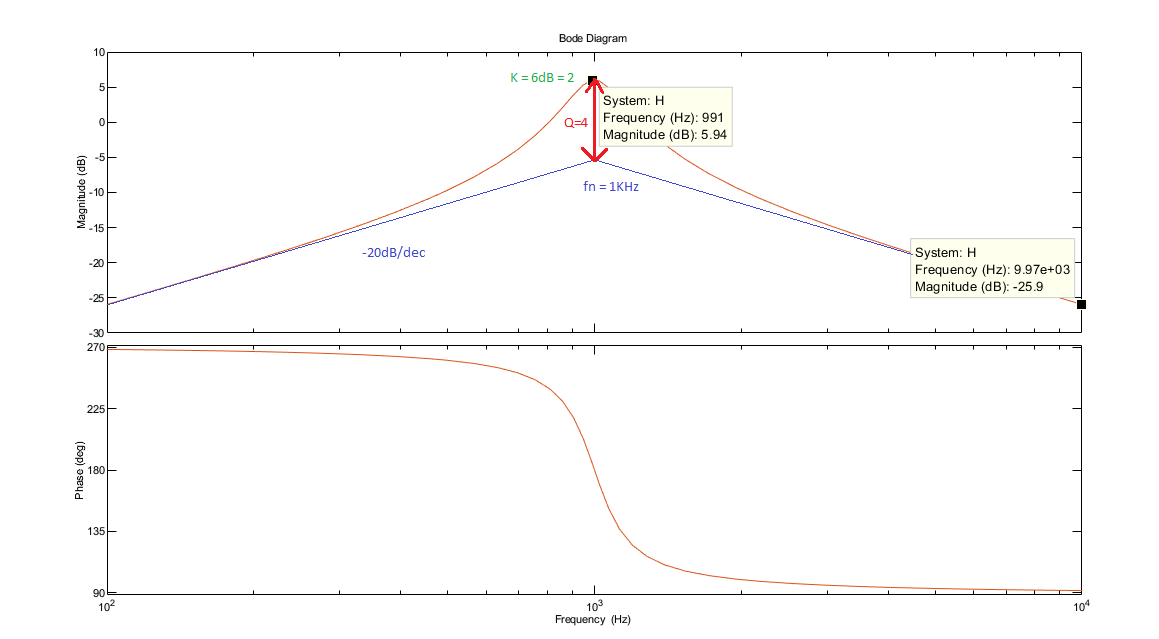
\includegraphics[width=13cm]{bode+freq}
\caption{Transferfunctie H(s) en Frequentiekarakteristiek}
\label{fig:bode+freq}
\end{figure}

\subsubsection*{Pole-Zero plot}

\begin{figure}[H]
\centering
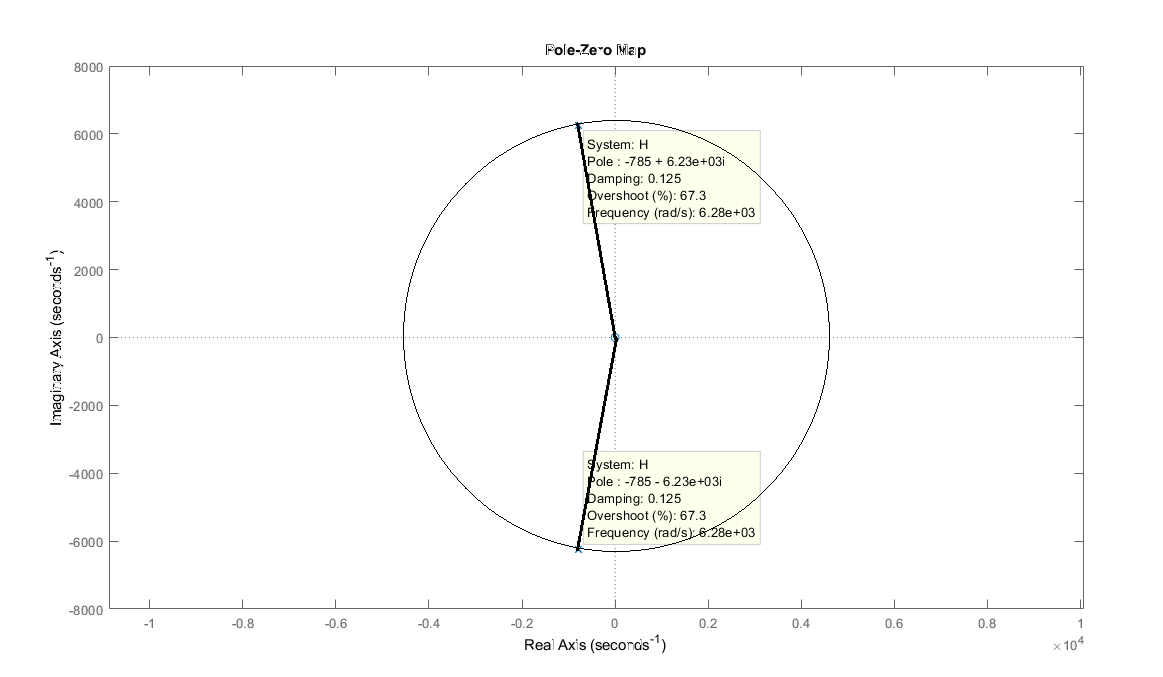
\includegraphics[width=13cm]{pz}
\caption{Pole-Zero plot}
\label{fig:pz}
\end{figure}

\subsubsection*{Stapresponsie}


\begin{figure}[H]
\centering
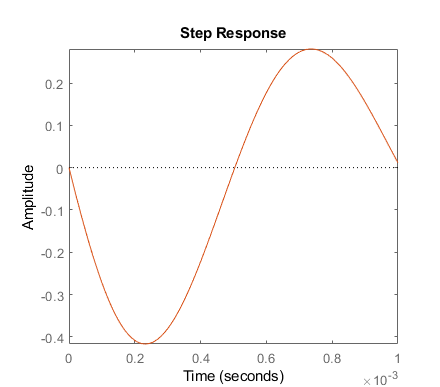
\includegraphics[width=9cm]{stap_1s}
\caption{Stapresponsie 1s}
\label{fig:pz}
\end{figure}

\begin{figure}[H]
\centering
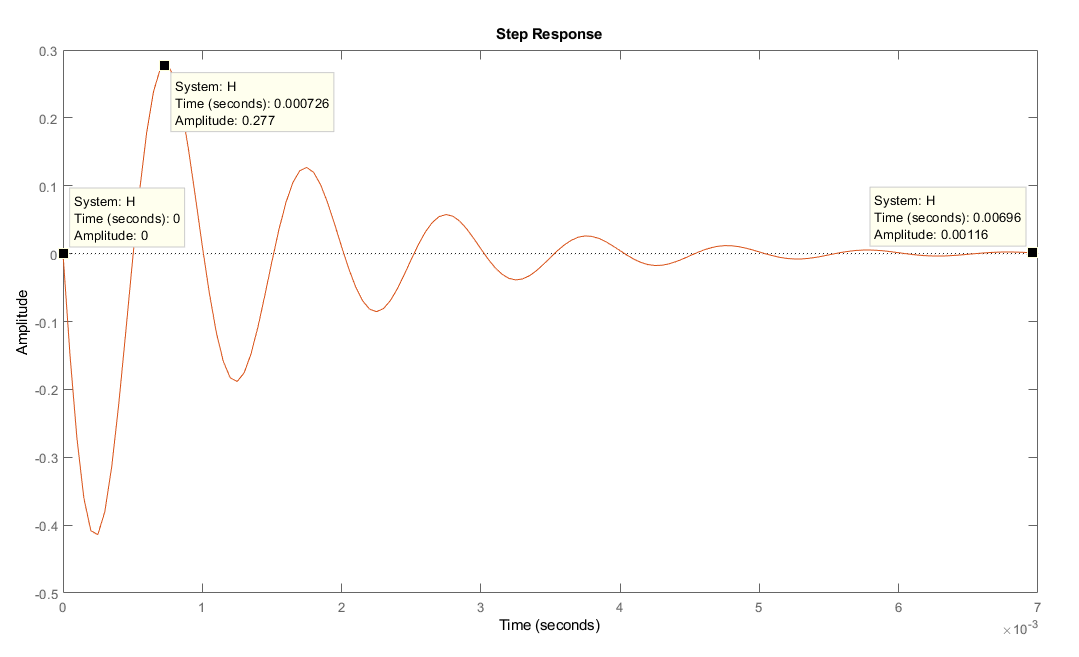
\includegraphics[width=13cm]{stap_7s}
\caption{Stapresponsie 7s}
\label{fig:pz}
\end{figure}

\section{Simulatie op basis van de netlijst (SPICE)}

\subsubsection*{Ideaal Opampmodel}

\begin{figure}[H]
	\centering
	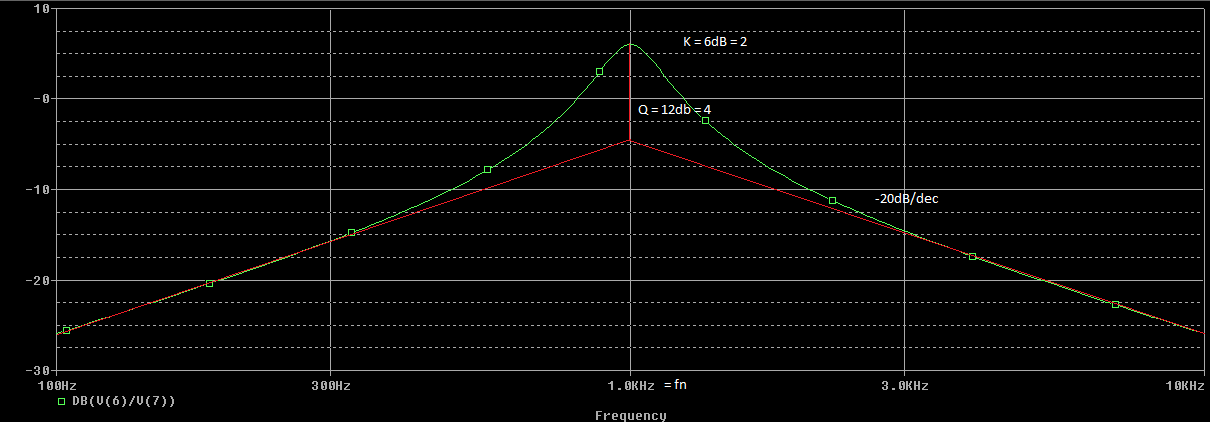
\includegraphics[width=13cm]{bode_ideaal_smal}
	\caption{Bode diagram ideal opamp model}
\end{figure}

\begin{figure}[H]
	\centering
	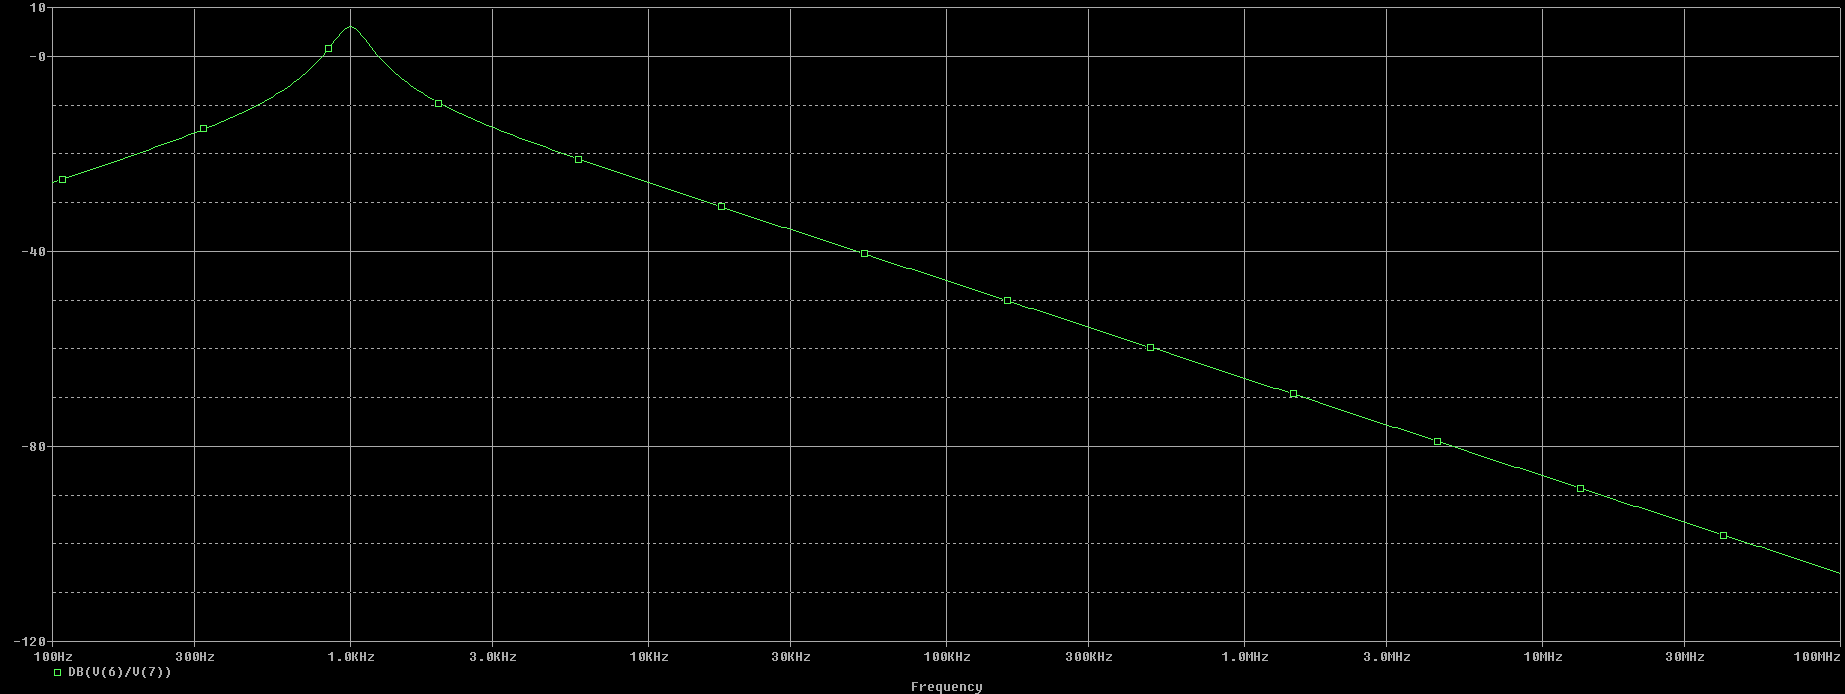
\includegraphics[width=13cm]{bode_ideaal}
	\caption{Bode diagram ideal opamp model HF}
\end{figure}

\begin{figure}[H]
	\centering
	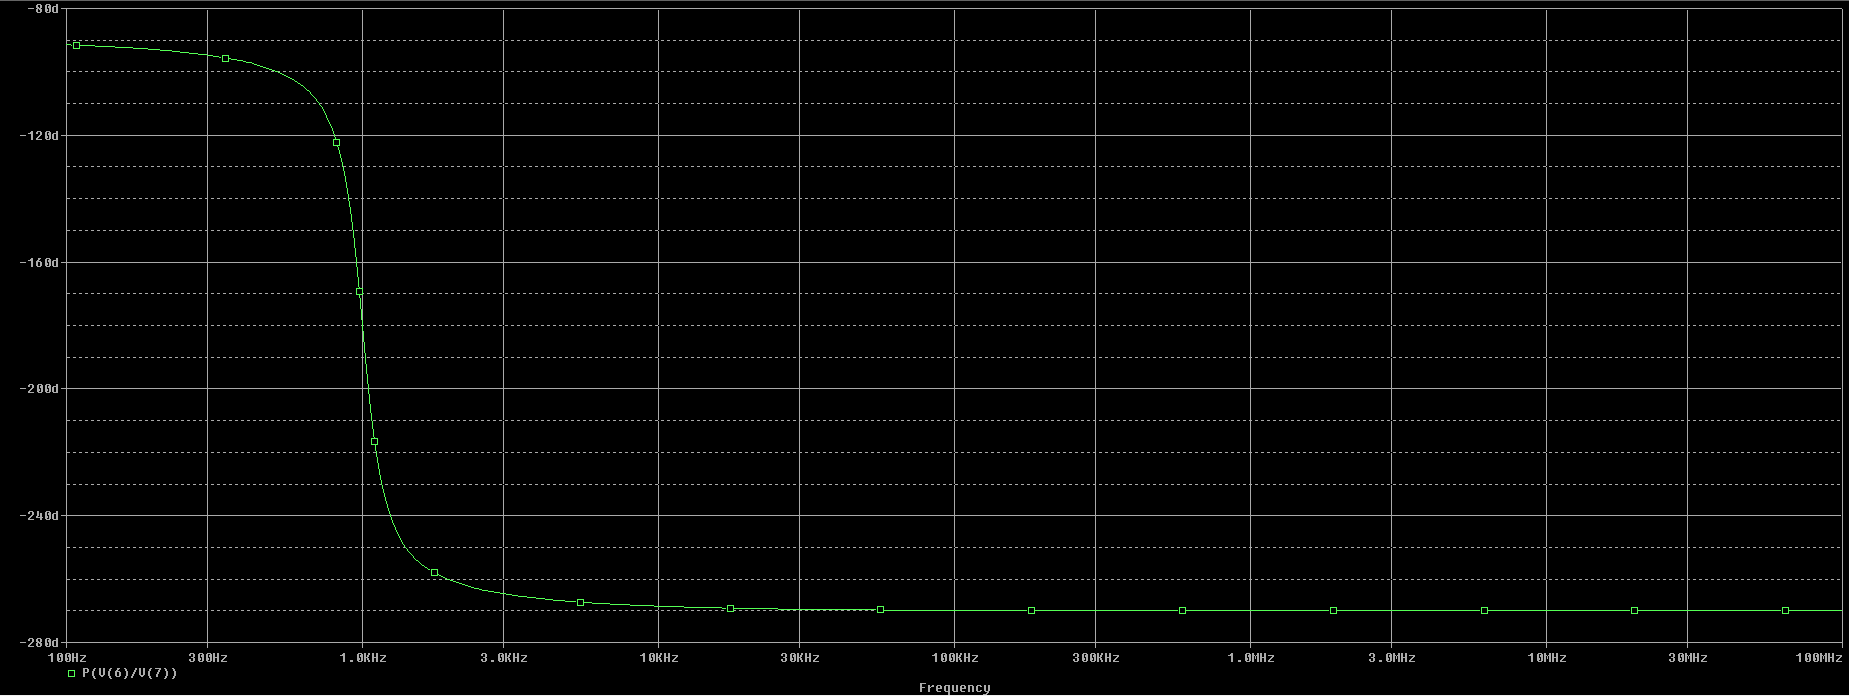
\includegraphics[width=13cm]{fase_ideaal}
	\caption{Fase diagram ideal opamp model HF}
\end{figure}

\newpage

\subsubsection*{VCVS}

\begin{figure}[H]
	\centering
	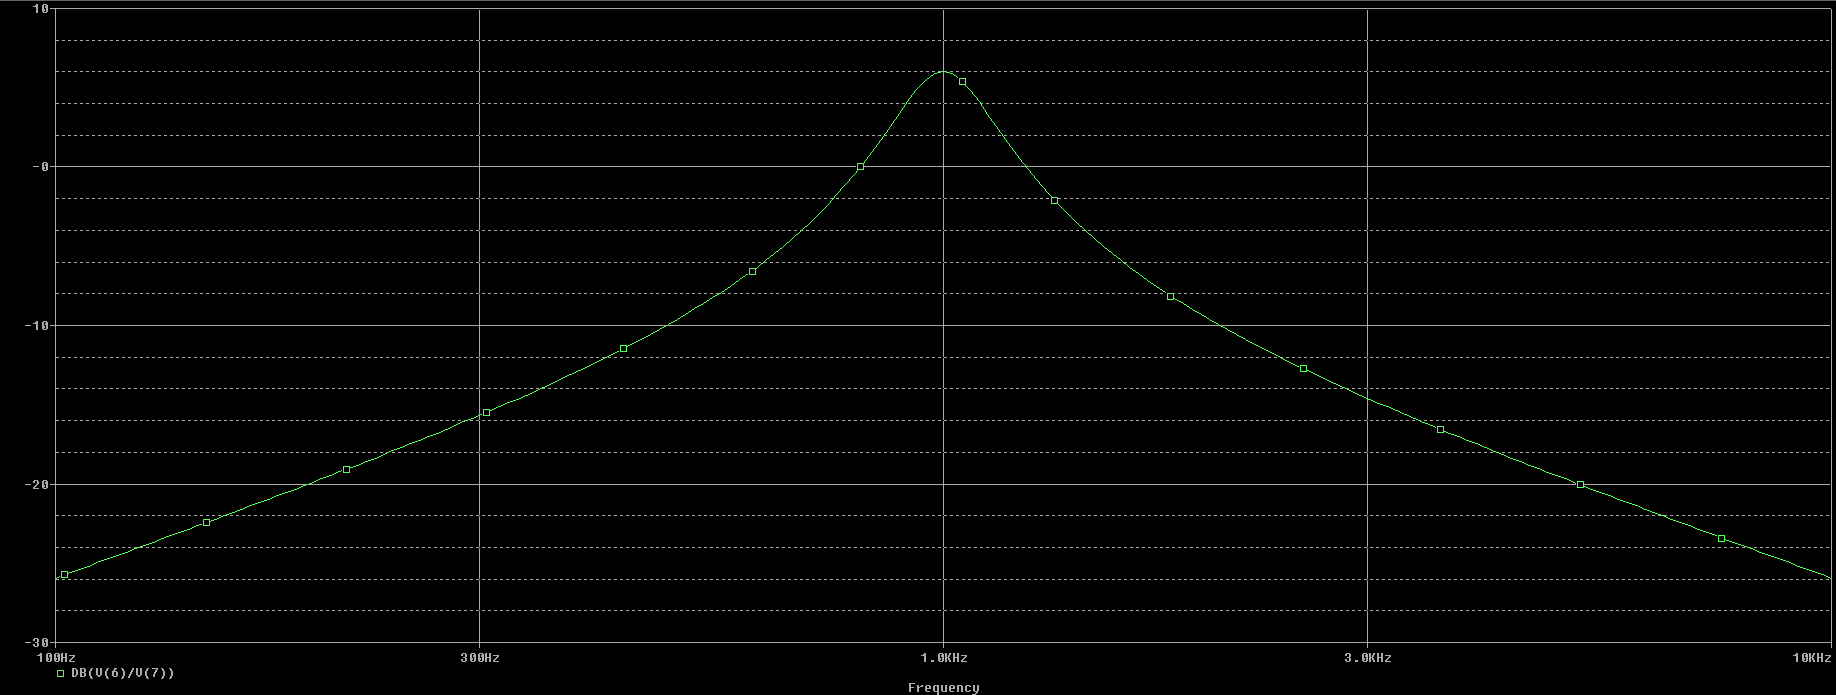
\includegraphics[width=13cm]{bode_vcvs_smal}
	\caption{Bode diagram vcvs opamp model}
\end{figure}

\begin{figure}[H]
	\centering
	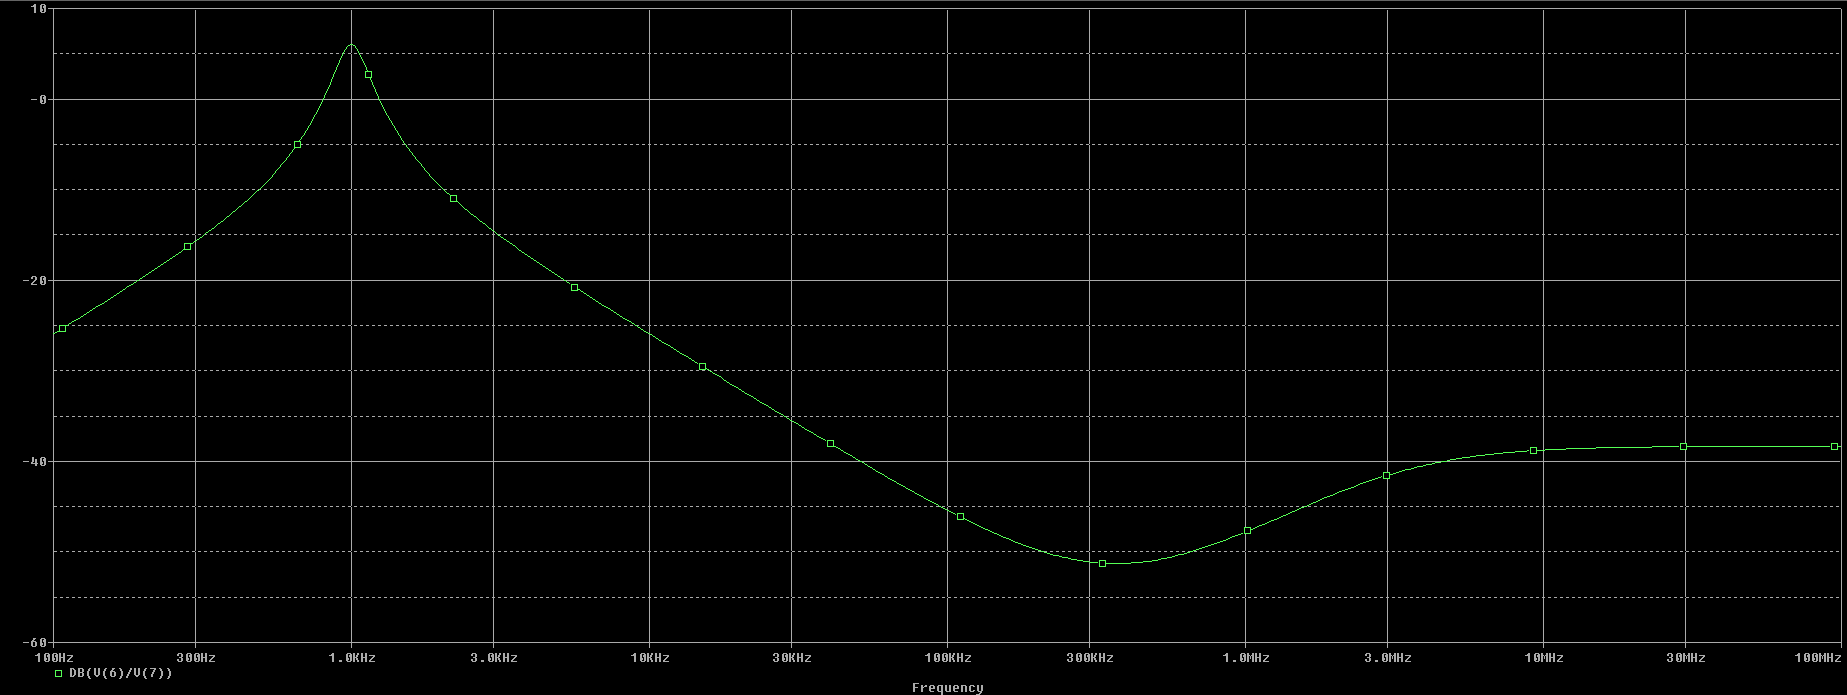
\includegraphics[width=13cm]{bode_vcvs}
	\caption{Bode diagram vcvs opamp model HF}
\end{figure}

Wanneer we het bodediagram verder in het frequentiedomein bekijken zien we dat de niet ideale opamp modellen vanaf een frequentie van 300KHz niet meer het verwachte filterpatroon vormen. Dit doordat we buiten het werkingsgebied van de opamp komen en er spanningsverliezen en faseverschuivingen optreden.

\begin{figure}[H]
	\centering
	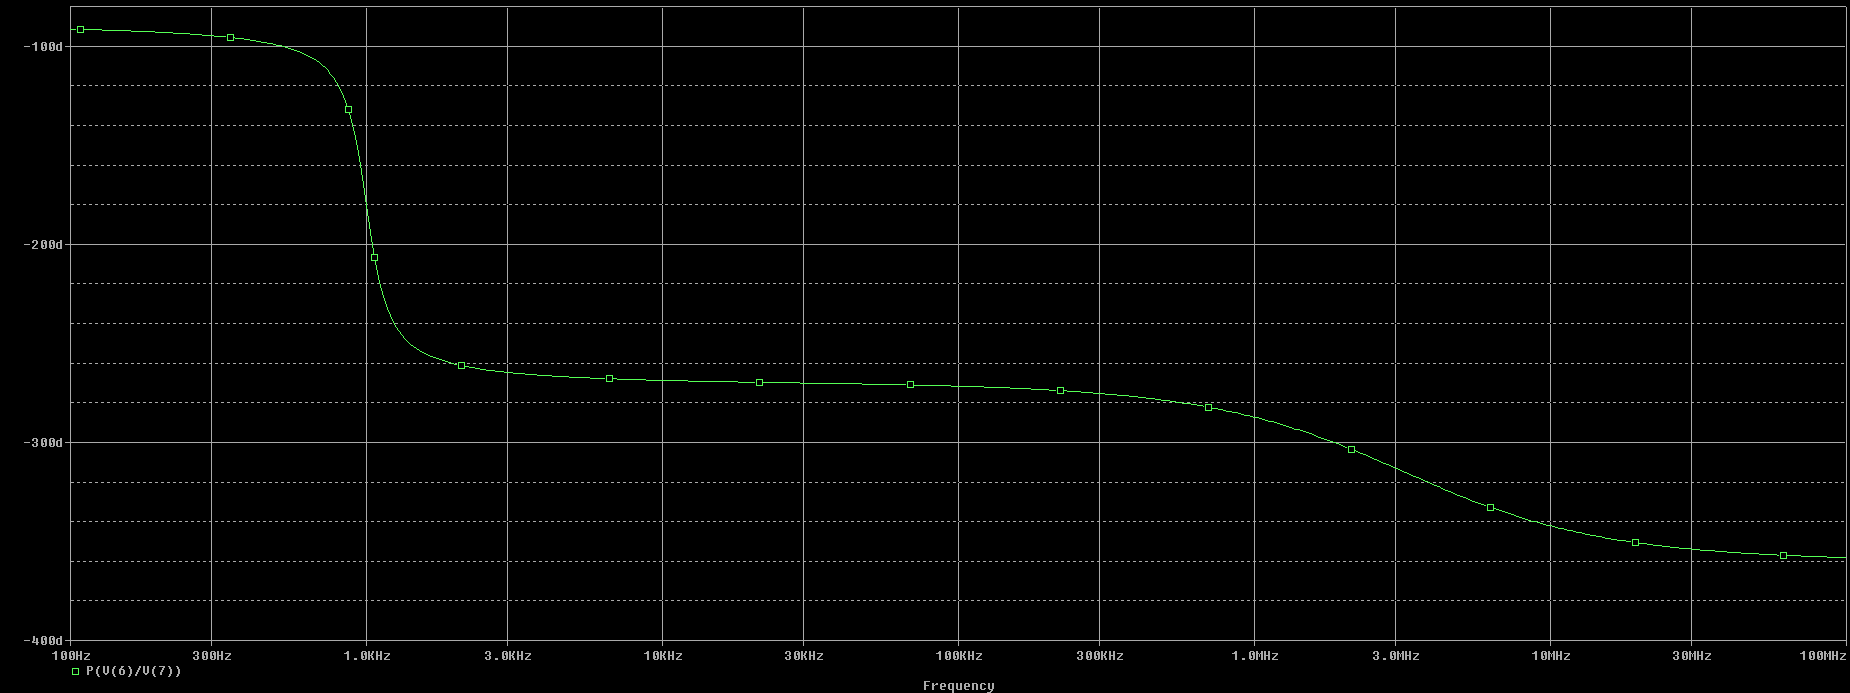
\includegraphics[width=13cm]{fase_vcvs}
	\caption{Fase diagram vcvs opamp model HF}
\end{figure}



\newpage

\subsubsection*{TL084}

\begin{figure}[H]
	\centering
	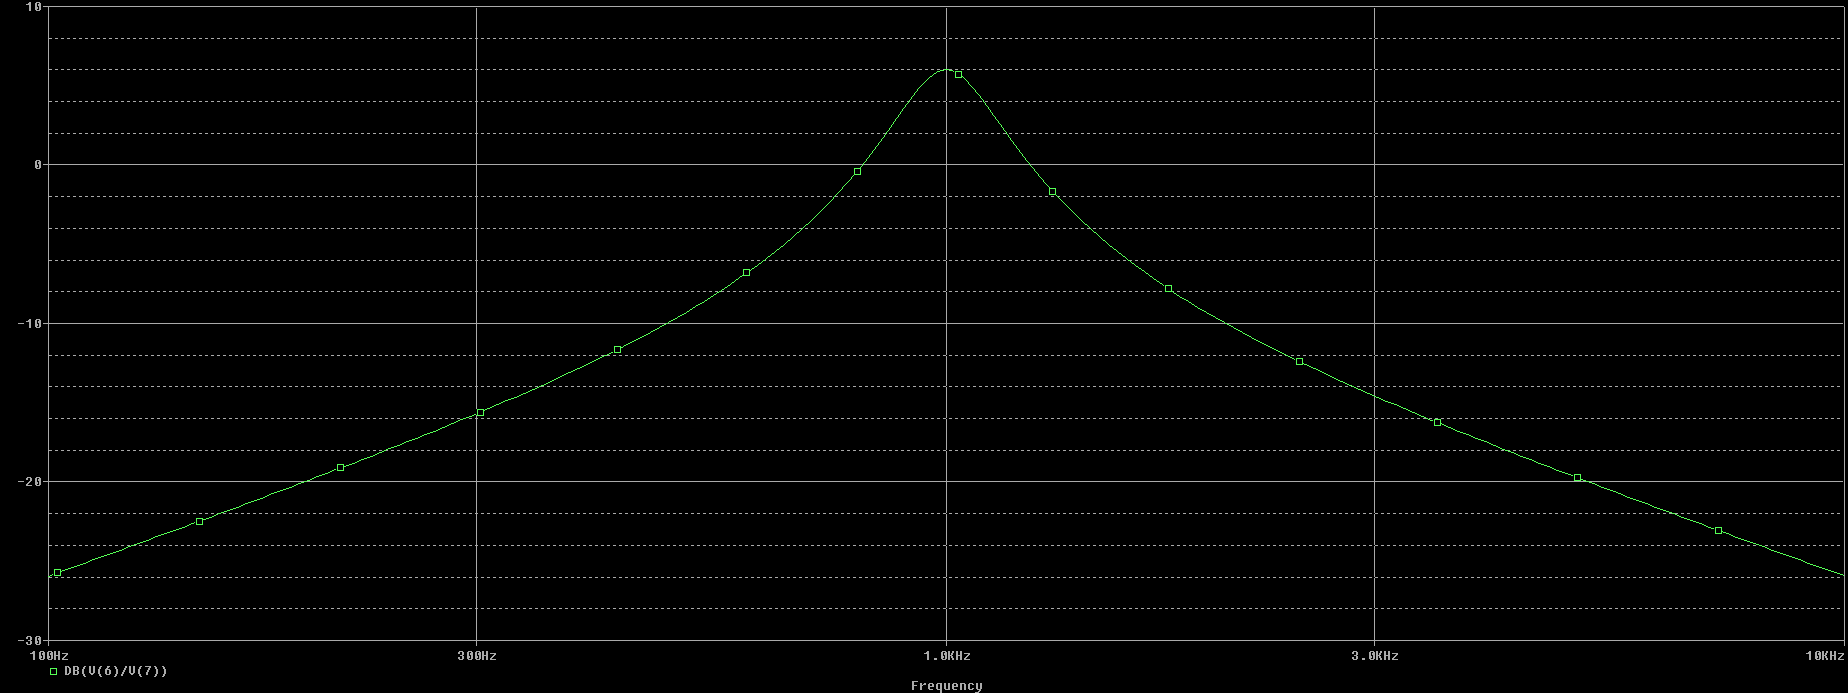
\includegraphics[width=13cm]{bode_TL084_smal}
	\caption{Bode diagram TL084 opamp model}
\end{figure}

\begin{figure}[H]
	\centering
	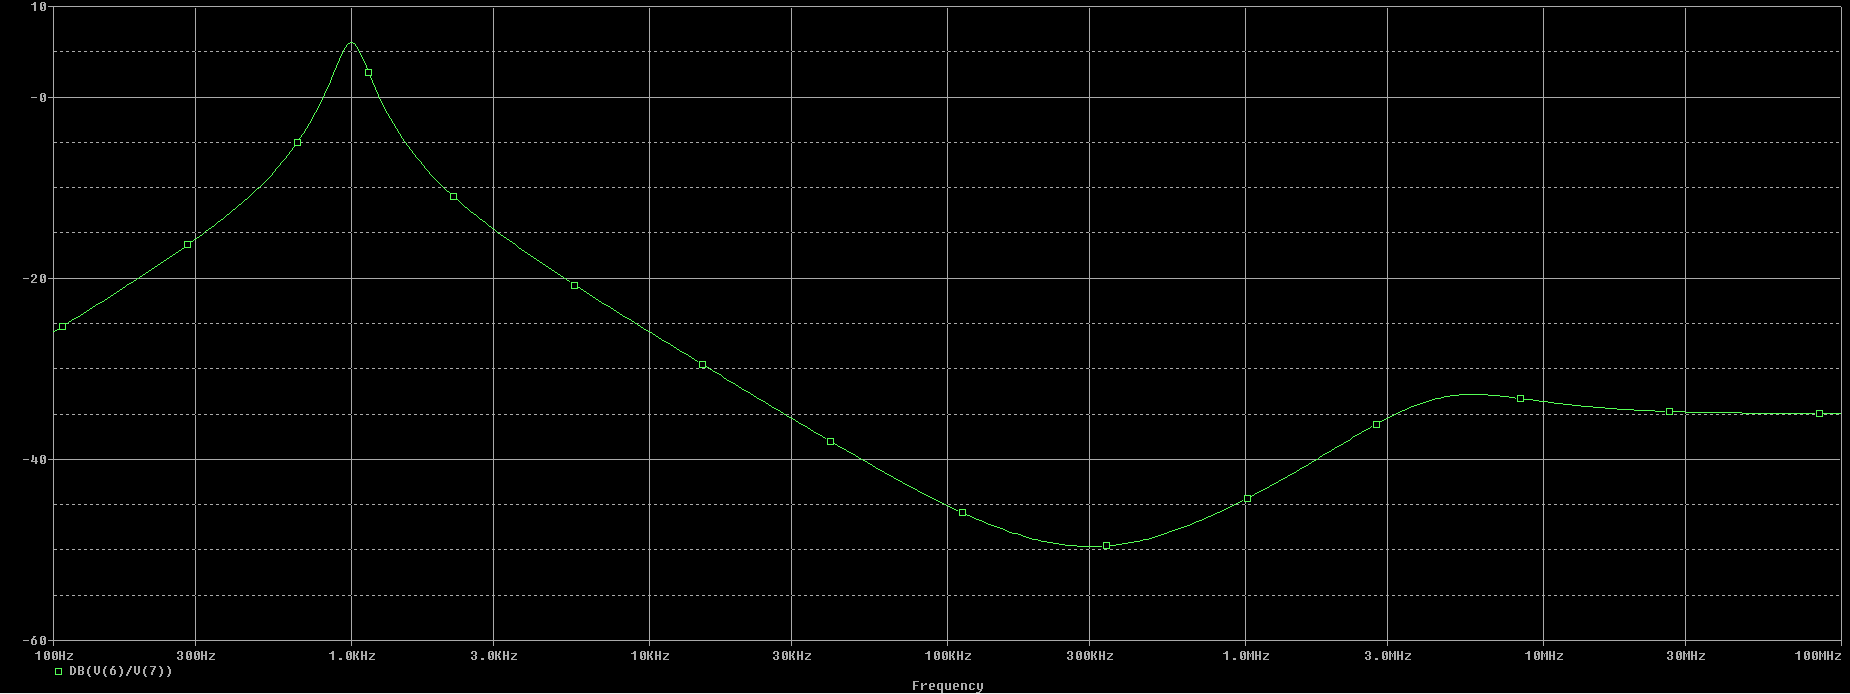
\includegraphics[width=13cm]{bode_TL084}
	\caption{Bode diagram TL084 opamp model HF}
\end{figure}

\begin{figure}[H]
	\centering
	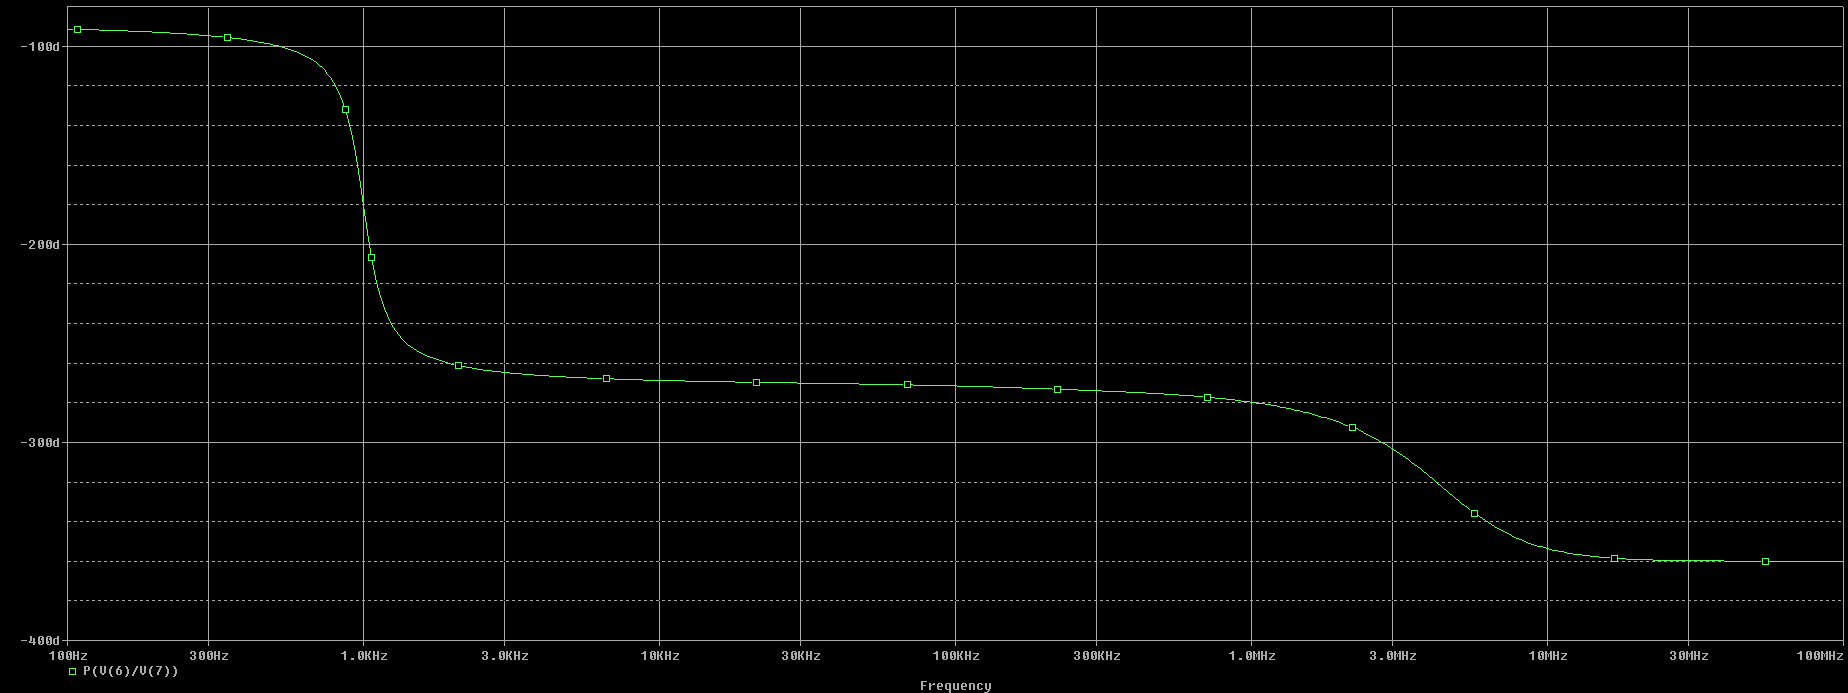
\includegraphics[width=13cm]{fase_TL084}
	\caption{Fase diagram TL084 opamp model HF}
\end{figure}

\newpage

\subsubsection*{Monte Carlo Anlayse}

\begin{figure}[H]
	\centering
	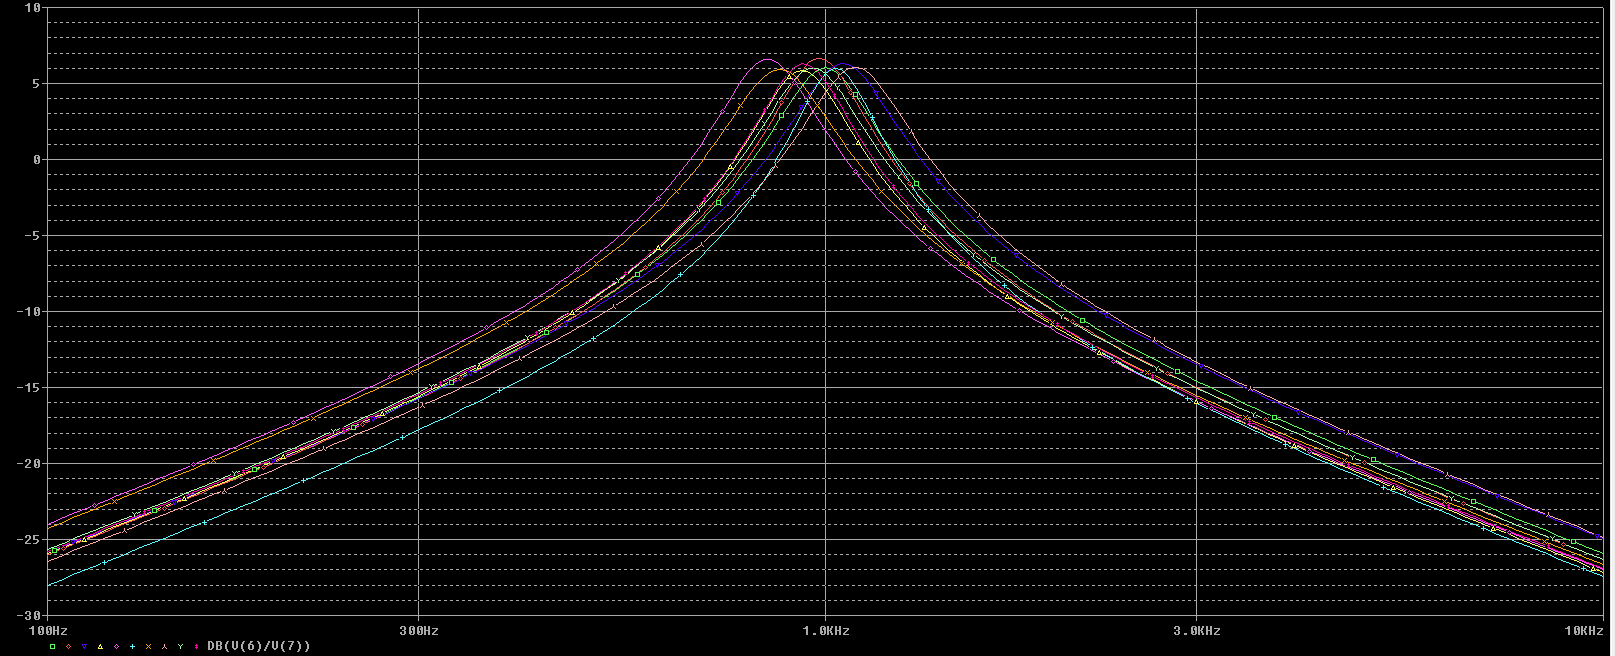
\includegraphics[width=13cm]{mc_transfer_smal}
	\caption{Monte Carlo Analyse R=5\% C=20\%}
	\label{fig:mc_transfer_smal}
\end{figure}

\begin{figure}[H]
	\centering
	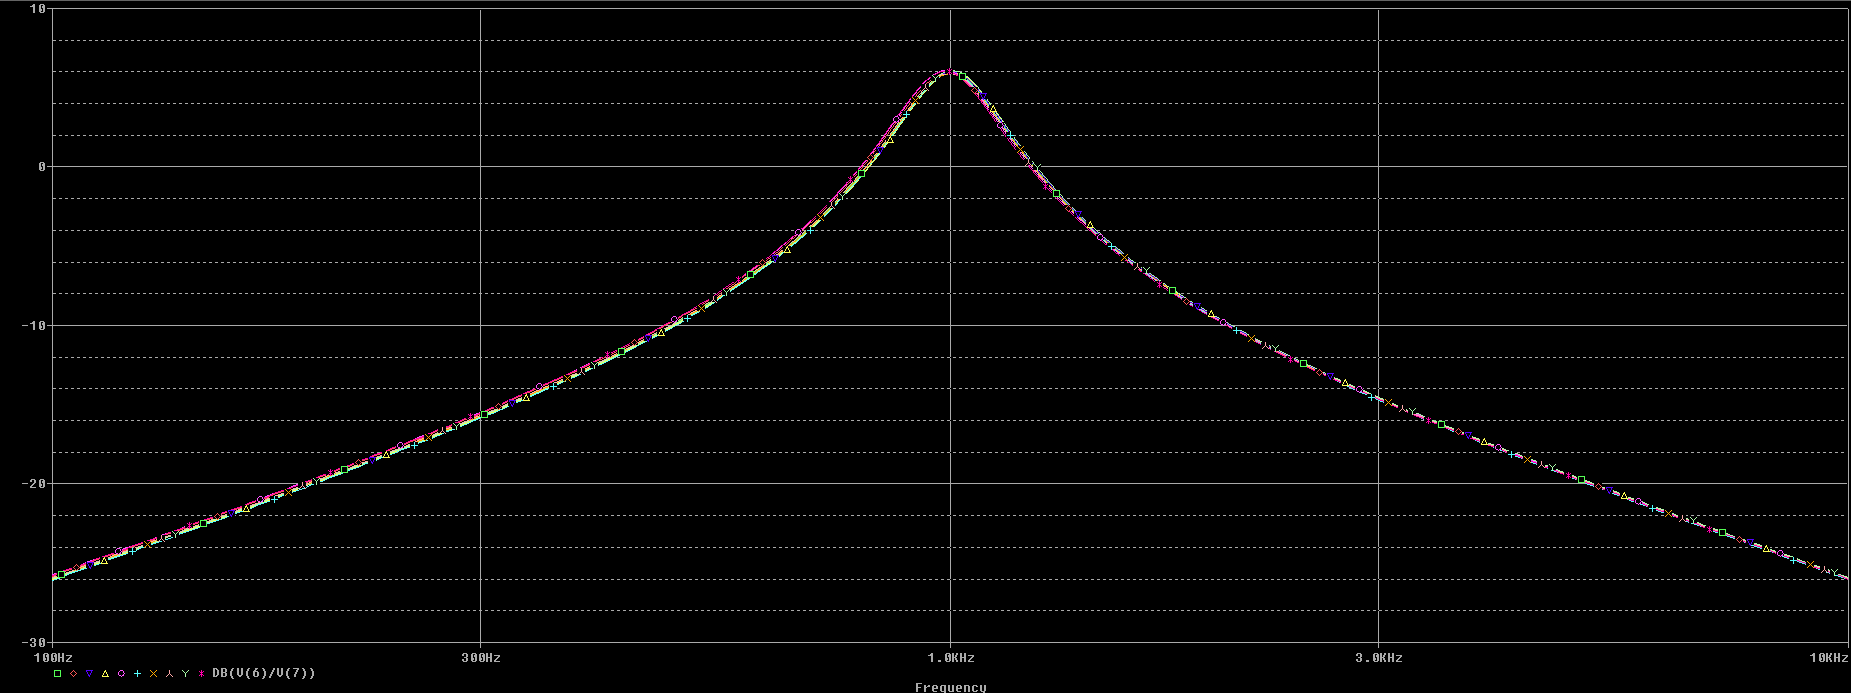
\includegraphics[width=13cm]{mc1}
	\caption{Monte Carlo Analyse R=1\% C=1\%}
	\label{fig:mc_transfer}
\end{figure}

\newpage

\subsubsection*{Ingangsimpedantie}

Op onderstaande figuur zien we de ingangsimpedantie van het circuit. We merken op dat deze vrij constant is met een lichte variatie rond 7.96K$\Omega$. Enkel rond de natuurlijke pulsatie zien we de ingangsimpedantie licht varieren, maar deze schommelingen zijn vrij klein. We kunnen dus zeggen da de ingangsimpedantie over de voledige lijn resistief is. Het licht naar beneden gaan wijst op een capacitief karakter, het licht naar boven gaan op een inductief karakter. Echter zijn deze schommelingen te verwaarlozen. 

\begin{figure}[H]
	\centering
	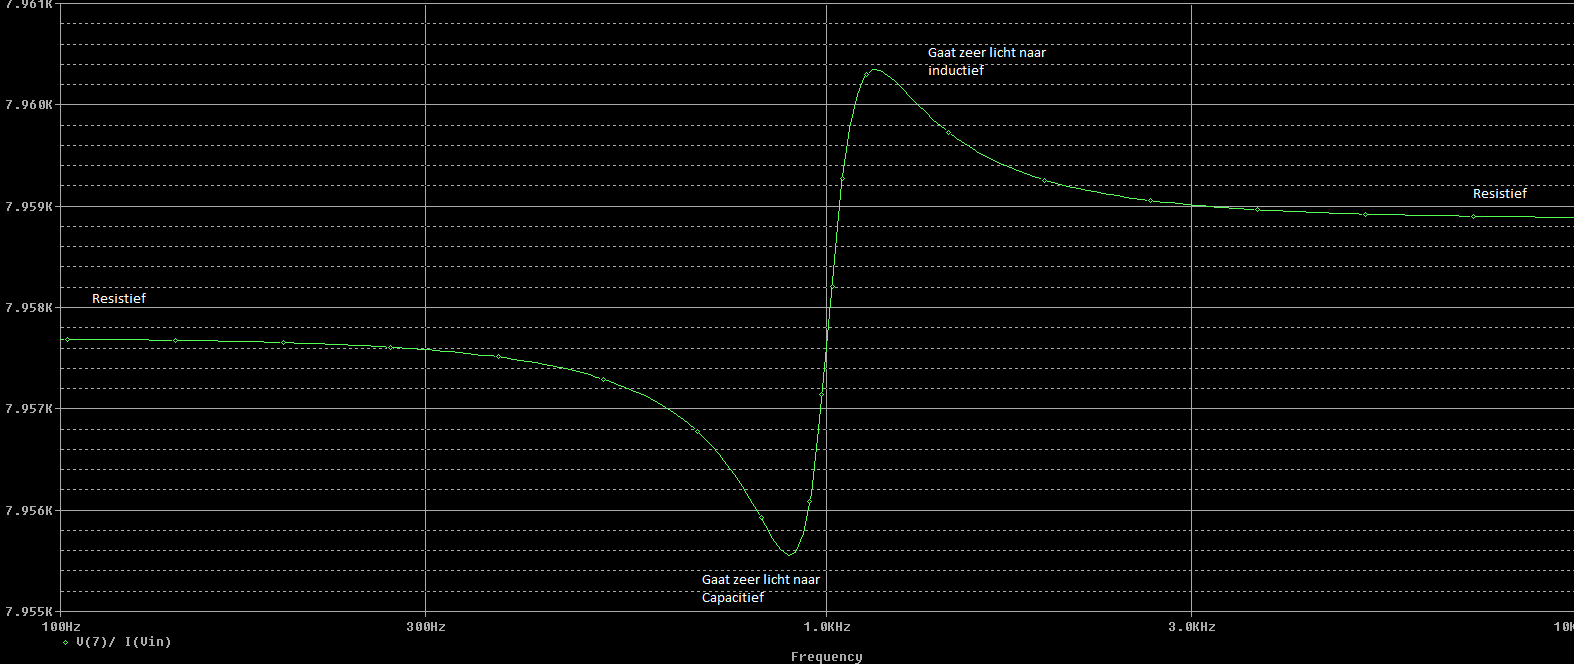
\includegraphics[width=13cm]{ingangsimp}
	\caption{Ingangsimpedantie}
	\label{fig:ingangsimp}
\end{figure}

\subsubsection*{Stapresponsie}

\begin{figure}[H]
	\centering
	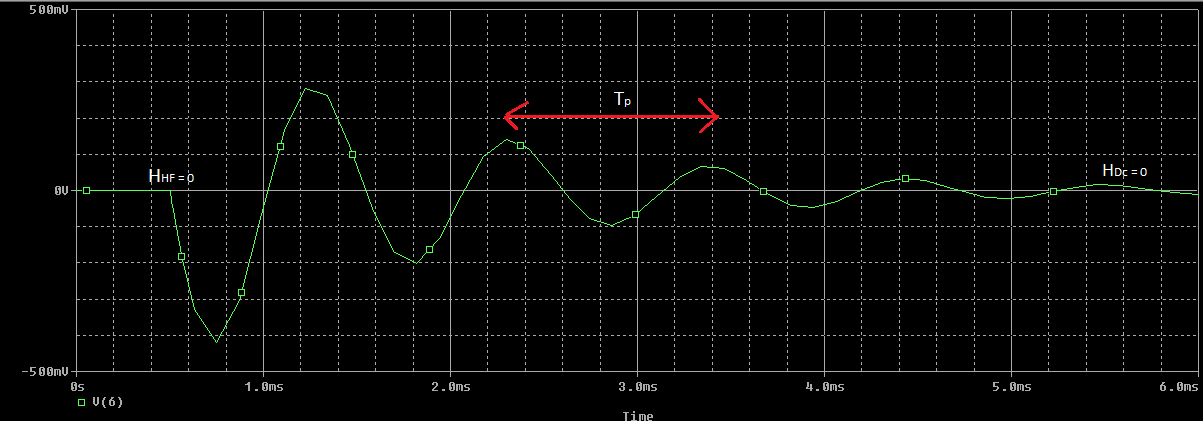
\includegraphics[width=13cm]{stap}
	\caption{Stapresponsie}
	\label{fig:stap}
\end{figure}


\end{document}
